\documentclass{article}
\iffalse
This file is protected by Copyright. Please refer to the COPYRIGHT file
distributed with this source distribution.

This file is part of OpenCPI <http://www.opencpi.org>

OpenCPI is free software: you can redistribute it and/or modify it under the
terms of the GNU Lesser General Public License as published by the Free Software
Foundation, either version 3 of the License, or (at your option) any later
version.

OpenCPI is distributed in the hope that it will be useful, but WITHOUT ANY
WARRANTY; without even the implied warranty of MERCHANTABILITY or FITNESS FOR A
PARTICULAR PURPOSE. See the GNU Lesser General Public License for more details.

You should have received a copy of the GNU Lesser General Public License along
with this program. If not, see <http://www.gnu.org/licenses/>.
\fi

\author{} % Force author to be blank
%----------------------------------------------------------------------------------------
% Paper size, orientation and margins
%----------------------------------------------------------------------------------------
\usepackage{geometry}
\geometry{
	letterpaper,			% paper type
	portrait,				% text direction
	left=.75in,				% left margin
	top=.75in,				% top margin
	right=.75in,			% right margin
	bottom=.75in			% bottom margin
 }
%----------------------------------------------------------------------------------------
% Header/Footer
%----------------------------------------------------------------------------------------
\usepackage{fancyhdr} \pagestyle{fancy} % required for fancy headers
\renewcommand{\headrulewidth}{0.5pt}
\renewcommand{\footrulewidth}{0.5pt}
\rhead{\small{ANGRYVIPER Team}}
%----------------------------------------------------------------------------------------
% Appendix packages
%----------------------------------------------------------------------------------------
\usepackage[toc,page]{appendix}
%----------------------------------------------------------------------------------------
% Defined Commands & Renamed Commands
%----------------------------------------------------------------------------------------
\renewcommand{\contentsname}{Table of Contents}
\renewcommand{\listfigurename}{List of Figures}
\renewcommand{\listtablename}{List of Tables}
\newcommand{\todo}[1]{\textcolor{red}{TODO: #1}\PackageWarning{TODO:}{#1}} % To do notes
\newcommand{\code}[1]{\texttt{#1}} % For inline code snippet or command line
%----------------------------------------------------------------------------------------
% Various pacakges
%----------------------------------------------------------------------------------------
\usepackage{hyperref} % for linking urls and lists
\usepackage{graphicx} % for including pictures by file
\usepackage{listings} % for coding language styles
\usepackage{rotating} % for sideways table
\usepackage{pifont}   % for sideways table
\usepackage{pdflscape} % for landscape view
%----------------------------------------------------------------------------------------
% Table packages
%----------------------------------------------------------------------------------------
\usepackage{longtable} % for long possibly multi-page tables
\usepackage{tabularx} % c=center,l=left,r=right,X=fill
\usepackage{float}
\floatstyle{plaintop}
\usepackage[tableposition=top]{caption}
\newcolumntype{P}[1]{>{\centering\arraybackslash}p{#1}}
\newcolumntype{M}[1]{>{\centering\arraybackslash}m{#1}}
%----------------------------------------------------------------------------------------
% Block Diagram / FSM Drawings
%----------------------------------------------------------------------------------------
\usepackage{tikz}
\usetikzlibrary{shapes,arrows,fit,positioning}
\usetikzlibrary{automata} % used for the fsm
%----------------------------------------------------------------------------------------
% Colors Used
%----------------------------------------------------------------------------------------
\usepackage{colortbl}
\definecolor{blue}{rgb}{.7,.8,.9}
\definecolor{ceruleanblue}{rgb}{0.16, 0.32, 0.75}
\definecolor{drkgreen}{rgb}{0,0.6,0}
\definecolor{deepmagenta}{rgb}{0.8, 0.0, 0.8}
\definecolor{cyan}{rgb}{0.0,0.6,0.6}
\definecolor{maroon}{rgb}{0.5,0,0}
%----------------------------------------------------------------------------------------
% Update the docTitle and docVersion per document
%----------------------------------------------------------------------------------------
\def\docTitle{Component Data Sheet}
\def\docVersion{1.5}
%----------------------------------------------------------------------------------------
\date{Version \docVersion} % Force date to be blank and override date with version
\title{\docTitle}
\lhead{\small{\docTitle}}

\def\comp{rp\_cordic}
\edef\ecomp{rp_cordic}
\def\Comp{Rectangular to Polar CORDIC}
\graphicspath{ {figures/} }

\begin{document}

\section*{Summary - \Comp}
\begin{tabular}{|c|M{13.5cm}|}
	\hline
	\rowcolor{blue}
	                  &                                                    \\
	\hline
	Name              & \comp                                              \\
	\hline
	Worker Type       & Application                                        \\
	\hline
	Version           & v\docVersion \\
	\hline
	Release Date      & 4/2019 \\
	\hline
	Component Library & ocpi.assets.dsp\_comps                              \\
	\hline
	Workers           & \comp.hdl                                          \\
	\hline
	Tested Platforms  & xsim, isim, modelsim, alst4, ml605, ZedBoard(PL), Matchstiq-Z1(PL) \\
	\hline
\end{tabular}

\section*{Functionality}
\begin{flushleft}
	The Rectangular to Polar CORDIC (Coordinate Rotation Digital Computer) worker implements an FM Discriminator circuit as shown in Figure \ref{fig:fmd_circuit}. Complex samples are fed into the CORDIC, which output magnitude and phase values. A $d\phi$ circuit is applied to the phase to calculate real samples.
\end{flushleft}
{\centering\captionsetup{type=figure}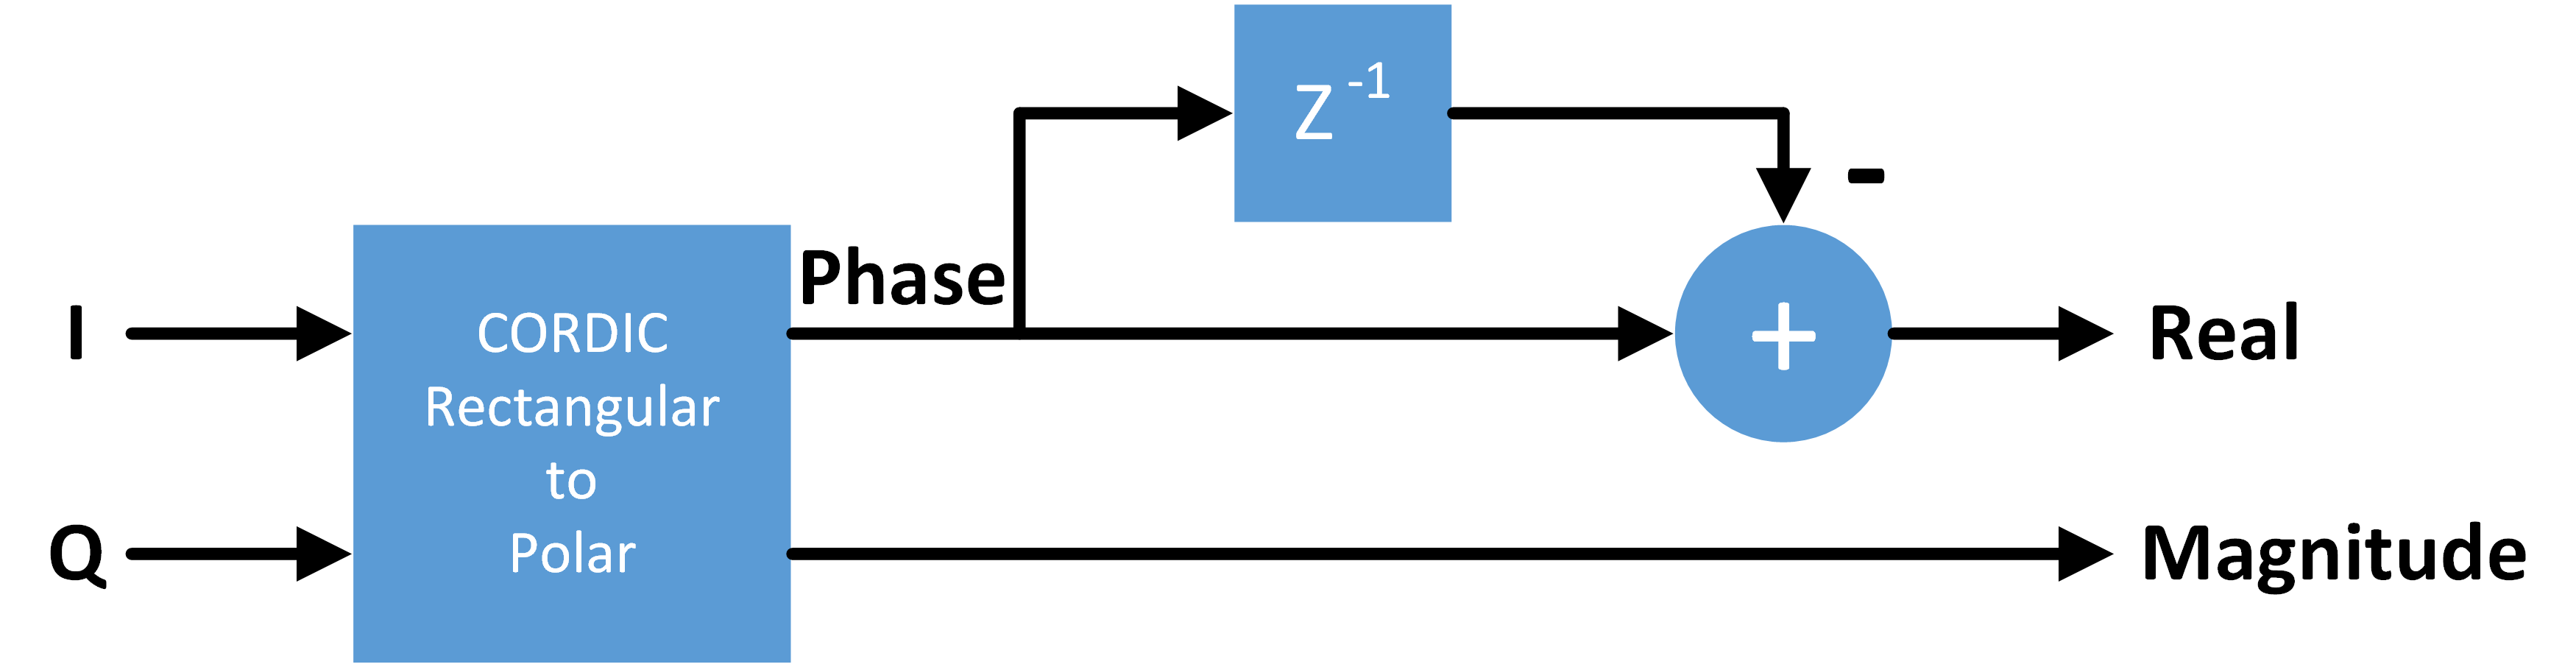
\includegraphics[scale=0.8]{fmd_circuit}\par\captionof{figure}{FM Discriminator Block Diagram}\label{fig:fmd_circuit}}

\section*{Worker Implementation Details}
\subsection*{\comp.hdl}
The FM Discriminator circuit consists of two sub-circuits: one to calculate the phase and another to calculate the rate of change of the phase. The first circuit uses a CORDIC algorithm to implement the arc-tangent function to calculate the phase of a complex sinusoid. The CORDIC is also used to calculate the magnitude of the complex sinusoid. Equations \ref{eq:1} and \ref{eq:2} represent the equations used to calculate the magnitude and phase, respectively. The magnitude output is exposed as a read-only property of the worker, which could be useful for downstream gain control.

\begin{equation} \label{eq:1}
	magnitude = \sqrt{I^2 + Q^2}
\end{equation}
\begin{equation} \label{eq:2}
	phase = atan(\frac{Q}{I})
\end{equation}

The second circuit simply uses a subtractor to implement a $d\phi$ function, which is a real signed number that is the difference in phase. Equations \ref{eq:3} and \ref{eq:4} show how to calculate $d\phi$.

\begin{equation} \label{eq:3}
	\omega = \frac{d\phi}{dt} = {2 \pi f}
\end{equation}
\begin{equation} \label{eq:4}
	d\phi = {2 \pi f dt} = {2 \pi f T_s} = \frac{2 \pi f}{F_s} = \frac{2 \pi f \frac{2^{DATAWIDTH-1}}{\pi}}{F_s} = \frac{2f*2^{DATAWIDTH-1}}{F_s}
\end{equation}
\newpage

\section*{Block Diagrams}
\subsection*{Top level}
\begin{center}
	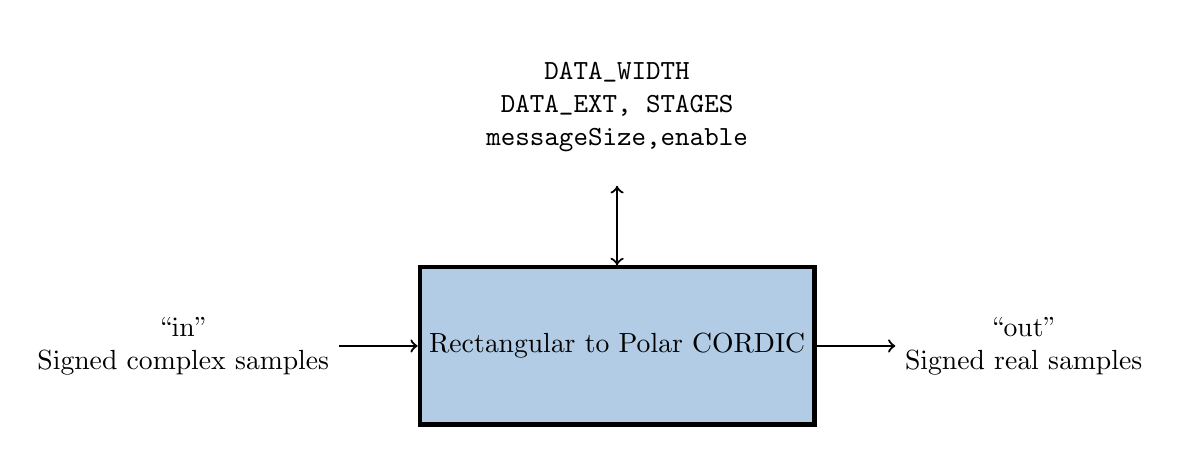
\begin{tikzpicture}[% List of styles applied to all, to override specify on a case-by-case
			every node/.style={
				align=center,  		% use this so that the "\\" for line break works
				minimum size=2cm	% creates space above and below text in rectangle
			},
			every edge/.style={draw,thick}
		]
		\node[rectangle,ultra thick,draw=black,fill=blue](R2){\Comp};
		\node[rectangle,draw=white,fill=white](R3)[left= of R2]{``in'' \\ Signed complex samples};
		\node[rectangle,draw=white,fill=white](R4)[right= of R2]{``out'' \\ Signed real samples};
		\node[rectangle,draw=white,fill=white](R5)[above= of R2]{\verb+DATA_WIDTH+ \\ \verb+DATA_EXT, STAGES+ \\ \verb+messageSize,enable+};
		\path[->]
		(R3)edge []	node [] {} (R2)
		(R2)edge []	node [] {} (R4)
		(R2)edge []	node [] {} (R5)
		(R5)edge []	node [] {} (R2)
		;
	\end{tikzpicture}
\end{center}

\subsection*{State Machine}
\begin{flushleft}
	Only one finite-state machine (FSM) is implemented by this worker. The FSM supports Zero-Length Messages.
\end{flushleft}
{\centering\captionsetup{type=figure}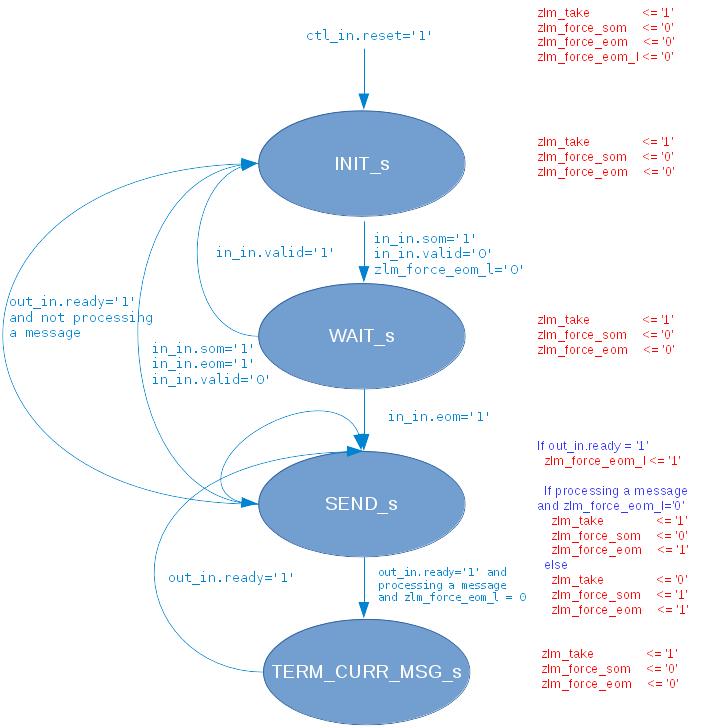
\includegraphics[scale=0.3]{rp_cordic_zlm_fsm}\par\captionof{figure}{Zero-Length Message FSM}\label{fig:rp_cordic_zlm_fsm}}
\begin{flushleft}
        Note: In future releases, this worker will be converted to the HDL version 2 API which will remove the need for this state machine.
\end{flushleft}


\newpage

\section*{Source Dependencies}
\subsection*{\comp.hdl}
\begin{itemize}
	\item projects/assets/components/dsp\_comps/rp\_cordic/rp\_cordic.vhd
	\item projects/assets/hdl/primitives/dsp\_prims/dsp\_prims\_pkg.vhd
	      \subitem projects/assets/hdl/primitives/dsp\_prims/cordic/src/cordic\_rp.vhd
	      \subitem projects/assets/hdl/primitives/dsp\_prims/cordic/src/cordic.vhd
	      \subitem projects/assets/hdl/primitives/dsp\_prims/cordic/src/cordic\_stage.vhd
	\item projects/assets/hdl/primitives/misc\_prims/misc\_prims\_pkg.vhd
	      \subitem projects/assets/hdl/primitives/misc\_prims/round\_conv/src/round\_conv.vhd
\end{itemize}

\begin{landscape}
	\section*{Component Spec Properties}
	\begin{scriptsize}
		\begin{tabular}{|p{3cm}|p{1.5cm}|c|c|c|c|c|p{7cm}|}
			\hline
			\rowcolor{blue}
			Name               & Type   & SequenceLength & ArrayDimensions & Accessibility      & Valid Range & Default & Usage                                        \\
			\hline
			\verb+DATA_WIDTH+  & UChar  & -              & -               & Readable           & -           & -       & Worker internal non-sign-extended data width \\
			\hline
			\verb+DATA_EXT+    & UChar  & -              & -               & Readable           & -           & -       & \# of extension bits                         \\
			\hline
			\verb+STAGES+      & UChar  & -              & -               & Readable           & -           & -       & Number of CORDIC stages implemented          \\
			\hline
			\verb+messageSize+ & UShort & -              & -               & Writable, Readable & 8192        & 8192    & Number of bytes in output message            \\
			\hline
			\verb+enable+      & Bool   & -              & -               & Writable, Readable & Standard    & true    & Enable/bypass control                        \\
			\hline
		\end{tabular}
	\end{scriptsize}

	\section*{Worker Properties}
	\subsection*{\comp.hdl}
	\begin{scriptsize}
		\begin{tabular}{|p{3cm}|p{2cm}|c|c|c|c|c|c|p{6cm}|}
			\hline
			\rowcolor{blue}
			Type         & Name              & Type  & SequenceLength & ArrayDimensions & Accessibility & Valid Range & Default & Usage                                                    \\
			\hline
			SpecProperty & \verb+DATA_WIDTH+ & -     & -              & -               & Parameter     & 8-16        & 16      & Real input and complex output data width                 \\
			\hline
			SpecProperty & \verb+DATA_EXT+   & -     & -              & -               & Parameter     & 6           & 6       & CORDIC requirement: \# of extension bits                 \\
			\hline
			SpecProperty & \verb+STAGES+     & -     & -              & -               & Parameter     & 8-16        & 16      & Number of CORDIC stages implemented                      \\
			\hline
			Property     & \verb+magnitude+  & Short & -              & -               & Volatile      & Standard    & -       & Read-only amplitude which may be useful for gain control \\
			\hline
		\end{tabular}
	\end{scriptsize}

	\section*{Component Ports}
	\begin{scriptsize}
		\begin{tabular}{|M{2cm}|M{1.5cm}|M{4cm}|c|c|M{9cm}|}
			\hline
			\rowcolor{blue}
			Name & Producer & Protocol           & Optional & Advanced & Usage                  \\
			\hline
			in   & false    & iqstream\_protocol & false    & -        & Signed complex samples \\
			\hline
			out  & true     & rstream\_protocol  & false    & -        & Signed real samples    \\
			\hline
		\end{tabular}
	\end{scriptsize}

	\section*{Worker Interfaces}
	\subsection*{\comp.hdl}
	\begin{scriptsize}
		\begin{tabular}{|M{2cm}|M{1.5cm}|c|c|M{12cm}|}
			\hline
			\rowcolor{blue}
			Type            & Name & DataWidth & Advanced                & Usage                  \\
			\hline
			StreamInterface & in   & 32        & ZeroLengthMessages=true & Signed complex samples \\
			\hline
			StreamInterface & out  & 16        & ZeroLengthMessages=true & Signed real samples    \\
			\hline
		\end{tabular}
	\end{scriptsize}
\end{landscape}

\section*{Control Timing and Signals}
The Rectangular to Polar CORDIC worker uses the clock from the Control Plane and standard Control Plane signals.

\noindent There is a start-up delay for this worker. Once the input is ready and valid and the output is ready, there is a delay of \verb+STAGES++4 before the first sample is taken. After this initial delay, valid output data is given \verb+STAGES++4 clock cycles after input data is taken.\medskip

\begin{tabular}{|M{4.5cm}|M{1cm}|M{1cm}|M{1.5cm}|M{2cm}|M{1cm}|M{1cm}|M{2.5cm}|}
	\hline
	\rowcolor{blue}
	Latency                      \\
	\hline
	\verb+STAGES++3 clock cycles \\
	\hline
\end{tabular}

\begin{landscape}
\section*{Worker Configuration Parameters}
\subsubsection*{\comp.hdl}
\input{../../\ecomp.hdl/configurations.inc}
\section*{Performance and Resource Utilization}
\subsubsection*{\comp.hdl}
\input{../../\ecomp.hdl/utilization.inc}
\end{landscape}
\section*{Test and Verification}
	One test case is implemented to validate the \Comp{} component:
	\begin{itemize}
		\item[1)] Normal mode
	\end{itemize}
	The input file is a waveform with a single tone at 27 Hz sampled at 10 kHz. The complex waveform is then scaled to fixed-point signed 16-bit integers, using a maximal amplitude of 32,767. Time and frequency domain plots may be viewed in Figures \ref{fig:in_time_tone} and \ref{fig:in_freq_tone} below, respectively.\par\medskip
	\begin{figure}[ht]
	\centering
	\begin{minipage}{.5\textwidth}
		\centering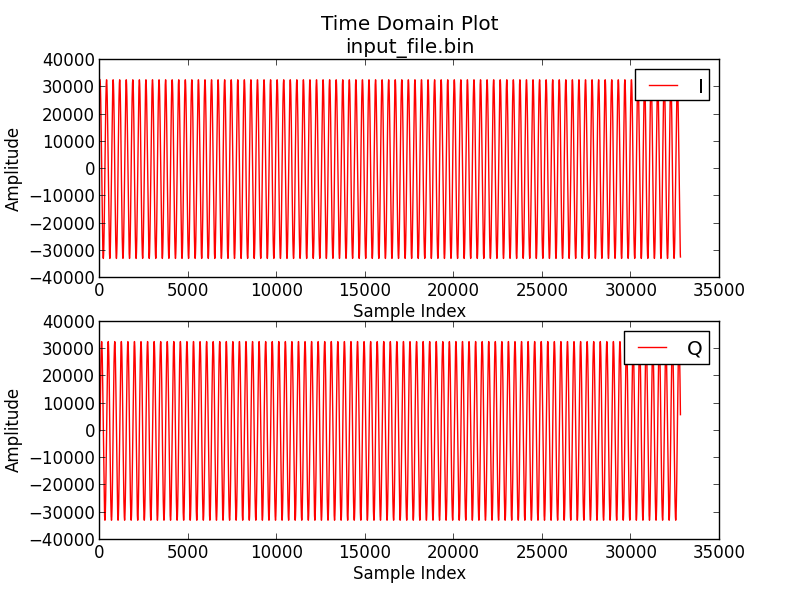
\includegraphics[width=1.0\linewidth]{input_time_tone}
		\captionof{figure}{Time Domain Complex Tone}
		\label{fig:in_time_tone}
	\end{minipage}%
	\begin{minipage}{.5\textwidth}
		\centering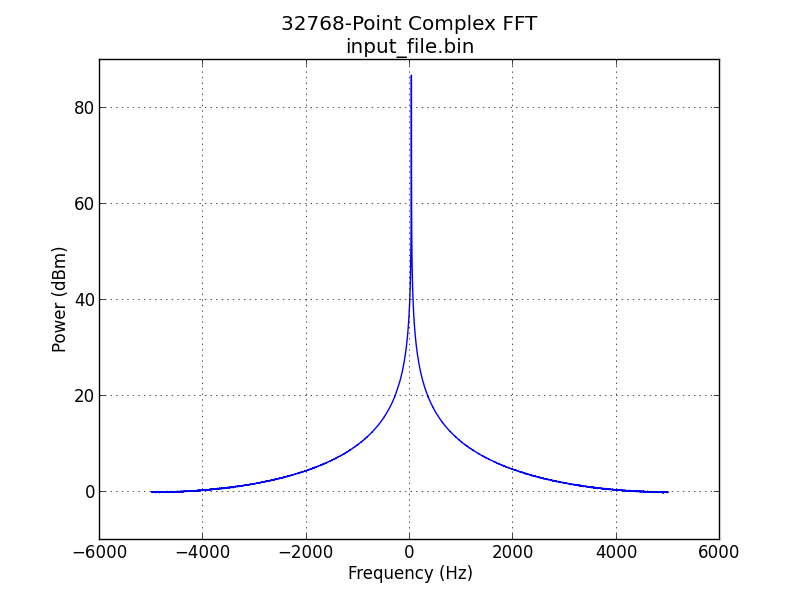
\includegraphics[width=1.0\linewidth]{input_freq_tone}
		\captionof{figure}{Frequency Domain Complex Tone}
		\label{fig:in_freq_tone}
	\end{minipage}
\end{figure}
	\noindent The output file is first checked that the data is not all zero and is then checked for the expected length. Once these quick checks are made, the complex input data is transformed into expected magnitude and phase arrays using Equations \ref{eq:1} and \ref{eq:2}. The expected phase array then implements the FM discriminator subtractor to create an array of the expected phase difference. These two expected value arrays are compared sample-by-sample with the measured phase output array from the UUT and the single value magnitude property from the UUT. Error checks are then calculated for the average peak error, the magnitude peak error, and the phase peak error. Should any of these three error values be more than one (the difference between each expected and measured value is allowed to be no greater than one) the overall test fails. Figure \ref{fig:out_time_real} depicts the conversion results of the single tone input, which shows no more than a $\pm1$ deviation from the expected result. Equation \ref{eq:4} is used to form Equation \ref{eq:5}, which validates the result shown in Figure \ref{fig:out_time_real}.

{\centering\captionsetup{type=figure}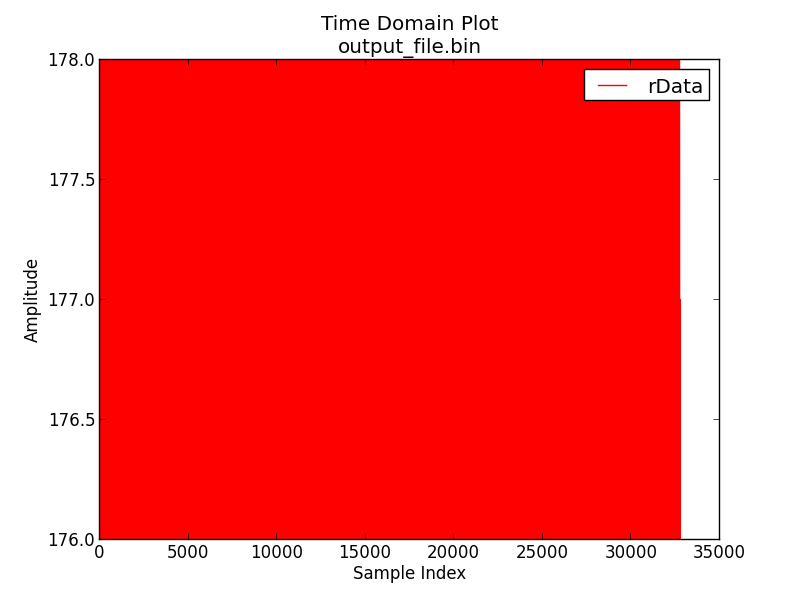
\includegraphics[scale=0.4]{output_time_real}\par\captionof{figure}{Time Domain Real Data}\label{fig:out_time_real}}

\begin{equation} \label{eq:5}
	d\phi = \frac{2f*2^{DATAWIDTH-1}}{F_s} = \frac{2*27*32,768}{10,000} = 176.9472
\end{equation}
\end{document}
